\documentclass[12pt,journal,compsoc]{IEEEtran}
\PassOptionsToPackage{spanish}{babel}
\usepackage{comment,graphicx,graphics, multicol}
\usepackage{babel}
\usepackage{dirtytalk}
\usepackage{enumitem}
\usepackage{minted}
\usepackage[table,xcdraw,usenames,dvipsnames]{xcolor}   % Colored text

% Background color for minted and text coloring style
\definecolor{codebg}{rgb}{0.95,0.95,0.95}
\usemintedstyle{friendly}

% Code enviroment. Escape with "@"
\newenvironment{code}[2]
 {\VerbatimEnvironment
  \begin{minted}[fontsize=#1, linenos,breaklines,numbersep=8pt,gobble=0,frame=lines,bgcolor=codebg,framesep=3mm,escapeinside=@@]{#2}}
 {\end{minted}}

 
% Palatino/Palladio as is done in IEEE Computer Society journals.
% To go back to Times Roman, you can use this code:
%\renewcommand{\rmdefault}{ptm}\selectfont

% *** CITATION PACKAGES ***
%
\ifCLASSOPTIONcompsoc
  % The IEEE Computer Society needs nocompress option
  % requires cite.sty v4.0 or later (November 2003)
  \usepackage[nocompress]{cite}
\else
  % normal IEEE
  \usepackage{cite}
\fi


% *** MATH PACKAGES ***
%
\usepackage{amsmath}
% A popular package from the American Mathematical Society that provides
% many useful and powerful commands for dealing with mathematics.
%
% Note that the amsmath package sets \interdisplaylinepenalty to 10000
% thus preventing page breaks from occurring within multiline equations. Use:
%\interdisplaylinepenalty=2500
% after loading amsmath to restore such page breaks as IEEEtran.cls normally
% does. amsmath.sty is already installed on most LaTeX systems. The latest
% version and documentation can be obtained at:
% http://www.ctan.org/pkg/amsmath


% *** SPECIALIZED LIST PACKAGES ***

\usepackage{algorithmic}
% algorithmic.sty was written by Peter Williams and Rogerio Brito.
% This package provides an algorithmic environment fo describing algorithms.
% You can use the algorithmic environment in-text or within a figure
% environment to provide for a floating algorithm. Do NOT use the algorithm
% floating environment provided by algorithm.sty (by the same authors) or
% algorithm2e.sty (by Christophe Fiorio) as the IEEE does not use dedicated
% algorithm float types and packages that provide these will not provide
% correct IEEE style captions. The latest version and documentation of
% algorithmic.sty can be obtained at:
% http://www.ctan.org/pkg/algorithms
% Also of interest may be the (relatively newer and more customizable)
% algorithmicx.sty package by Szasz Janos:
% http://www.ctan.org/pkg/algorithmicx


% *** ALIGNMENT PACKAGES ***
%
\usepackage{array}
% Frank Mittelbach's and David Carlisle's array.sty patches and improves
% the standard LaTeX2e array and tabular environments to provide better
% appearance and additional user controls. As the default LaTeX2e table
% generation code is lacking to the point of almost being broken with
% respect to the quality of the end results, all users are strongly
% advised to use an enhanced (at the very least that provided by array.sty)
% set of table tools. array.sty is already installed on most systems. The
% latest version and documentation can be obtained at:
% http://www.ctan.org/pkg/array


\usepackage{eqparbox}
% Also of notable interest is Scott Pakin's eqparbox package for creating
% (automatically sized) equal width boxes - aka "natural width parboxes".
% Available at:
% http://www.ctan.org/pkg/eqparbox


% *** PDF, URL AND HYPERLINK PACKAGES ***

% NOTE: PDF hyperlink and bookmark features are not required in IEEE
%       papers and their use requires extra complexity and work.
% *** IF USING HYPERREF BE SURE AND CHANGE THE EXAMPLE PDF ***
% *** TITLE/SUBJECT/AUTHOR/KEYWORDS INFO BELOW!!           ***
\newcommand\MYhyperrefoptions{bookmarks=true,bookmarksnumbered=true,
pdfpagemode={UseOutlines},plainpages=false,pdfpagelabels=true,
colorlinks=true,linkcolor={black},citecolor={black},urlcolor={black},
pdftitle={Bare Demo of IEEEtran.cls for Computer Society Journals},%<!CHANGE!
pdfsubject={Typesetting},%<!CHANGE!
pdfauthor={Michael D. Shell},%<!CHANGE!
pdfkeywords={Computer Society, IEEEtran, journal, LaTeX, paper,
             template}}%<^!CHANGE!
\ifCLASSINFOpdf
\usepackage[\MYhyperrefoptions,pdftex]{hyperref}
\else
\usepackage[\MYhyperrefoptions,breaklinks=true,dvips]{hyperref}
\usepackage{breakurl}
\fi
% One significant drawback of using hyperref under DVI output is that the
% LaTeX compiler cannot break URLs across lines or pages as can be done
% under pdfLaTeX's PDF output via the hyperref pdftex driver. This is
% probably the single most important capability distinction between the
% DVI and PDF output. Perhaps surprisingly, all the other PDF features
% (PDF bookmarks, thumbnails, etc.) can be preserved in
% .tex->.dvi->.ps->.pdf workflow if the respective packages/scripts are
% loaded/invoked with the correct driver options (dvips, etc.). 
% As most IEEE papers use URLs sparingly (mainly in the references), this
% may not be as big an issue as with other publications.
%
% That said, Vilar Camara Neto created his breakurl.sty package which
% permits hyperref to easily break URLs even in dvi mode.
% Note that breakurl, unlike most other packages, must be loaded
% AFTER hyperref. The latest version of breakurl and its documentation can
% be obtained at:
% http://www.ctan.org/pkg/breakurl
% breakurl.sty is not for use under pdflatex pdf mode.
%
% The advanced features offer by hyperref.sty are not required for IEEE
% submission, so users should weigh these features against the added
% complexity of use.
% The package options above demonstrate how to enable PDF bookmarks
% (a type of table of contents viewable in Acrobat Reader) as well as
% PDF document information (title, subject, author and keywords) that is
% viewable in Acrobat reader's Document_Properties menu. PDF document
% information is also used extensively to automate the cataloging of PDF
% documents. The above set of options ensures that hyperlinks will not be
% colored in the text and thus will not be visible in the printed page,
% but will be active on "mouse over". USING COLORS OR OTHER HIGHLIGHTING
% OF HYPERLINKS CAN RESULT IN DOCUMENT REJECTION BY THE IEEE, especially if
% these appear on the "printed" page. IF IN DOUBT, ASK THE RELEVANT
% SUBMISSION EDITOR. You may need to add the option hypertexnames=false if
% you used duplicate equation numbers, etc., but this should not be needed
% in normal IEEE work.
% The latest version of hyperref and its documentation can be obtained at:
% http://www.ctan.org/pkg/hyperref

% correct bad hyphenation here
\hyphenation{op-tical net-works semi-conduc-tor}
\usepackage{csquotes}

\begin{document}

% PAPER HEADER 
\markboth{GEIN-3, Algoritmos avanzados, Práctica 7, \today}{}
% The only time the second header will appear is for the odd numbered pages
% after the title page when using the twoside option.
% 
% *** Note that you probably will NOT want to include the author's ***
% *** name in the headers of peer review papers.                   ***

% PAPER TITLE 
\title{Primalidad y Encriptación RSA}
% Titles are generally capitalized except for words such as a, an, and, as,
% at, but, by, for, in, nor, of, on, or, the, to and up, which are usually
% Do not put math or special symbols in the title.

% PAPER AUTHORS
\author{Alejandro Rodríguez, Rubén Palmer y Sergi Mayol}

% for Computer Society papers, we must declare the abstract and index terms
% As a general rule, do not put math, special symbols or citations in the abstract or keywords.
\IEEEtitleabstractindextext{%
\begin{abstract}
\hspace{2pt}
Esta aplicación presenta una interfáz gráfica de usuario que permite identificar la primalidad y los factores de un número arbitrariamente grande. Adicionalmente, hay un \say{playground} donde el usuario puede encriptar, desencriptar y guardar textos mediante claves RSA de tamaño variable.
\end{abstract}

{\scriptsize \textbf{Vídeo} - \href{https://youtu.be/6WhkiI0S3Us}{\textcolor{blue}{ver vídeo}}}
}

% make the title area
\maketitle
\IEEEdisplaynontitleabstractindextext
\IEEEpeerreviewmaketitle

% IEEEraisesectionheading removes all the unnecesary space between the first instance of the paper and the title
\IEEEraisesectionheading{\section{Introducción}\label{sec:introduction}}

% The very first letter is a 2 line initial drop letter followed
% by the rest of the first word in caps (small caps for compsoc).
% 
% form to use if the first word consists of a single letter:
% \IEEEPARstart{A}{demo} file is ....
% 
\IEEEPARstart{E}{n} este artículo explicaremos el funcionamiento y la implementación de nuestra práctica estructurando y dividiendo sus partes en los siguientes apartados:\bigskip

Inicialmente, se citarán las librerías usadas en este proyecto. Para aquellas que se hayan desarrollado específicamente, se expondrá una breve guía de su funcionamiento y uso.\bigskip

Seguidamente, se explicará cuál es la arquitectura, interfaces, funcionamiento e implementación de nuestro \textbf{M}odelo-\textbf{V}ista-\textbf{C}ontrolador (MVC) así como los métodos de mayor importancia. Para facilitar la legibilidad, se separará en cada uno de los grandes bloques de la estructura; en este caso Modelo, Vista, Controlador y Hub\bigskip

Finalmente, se mostrará una breve guía de cómo usar nuestra aplicación y un ejemplo de esta.

\section{Manual de usuario}\label{Manual usuario}

Para el correcto uso de la aplicación, el conjunto de acciones que se pueden realizar en dicho programa serán definidas a continuación. También, la distribución de las secciones de la interfaz junto a su explicación y funcionalidad.\bigskip

Cuando se ejecute el programa por primera vez en la pantalla se debe mostrar la siguiente interfaz de usuario:

\begin{figure}[!h]
    \centering
    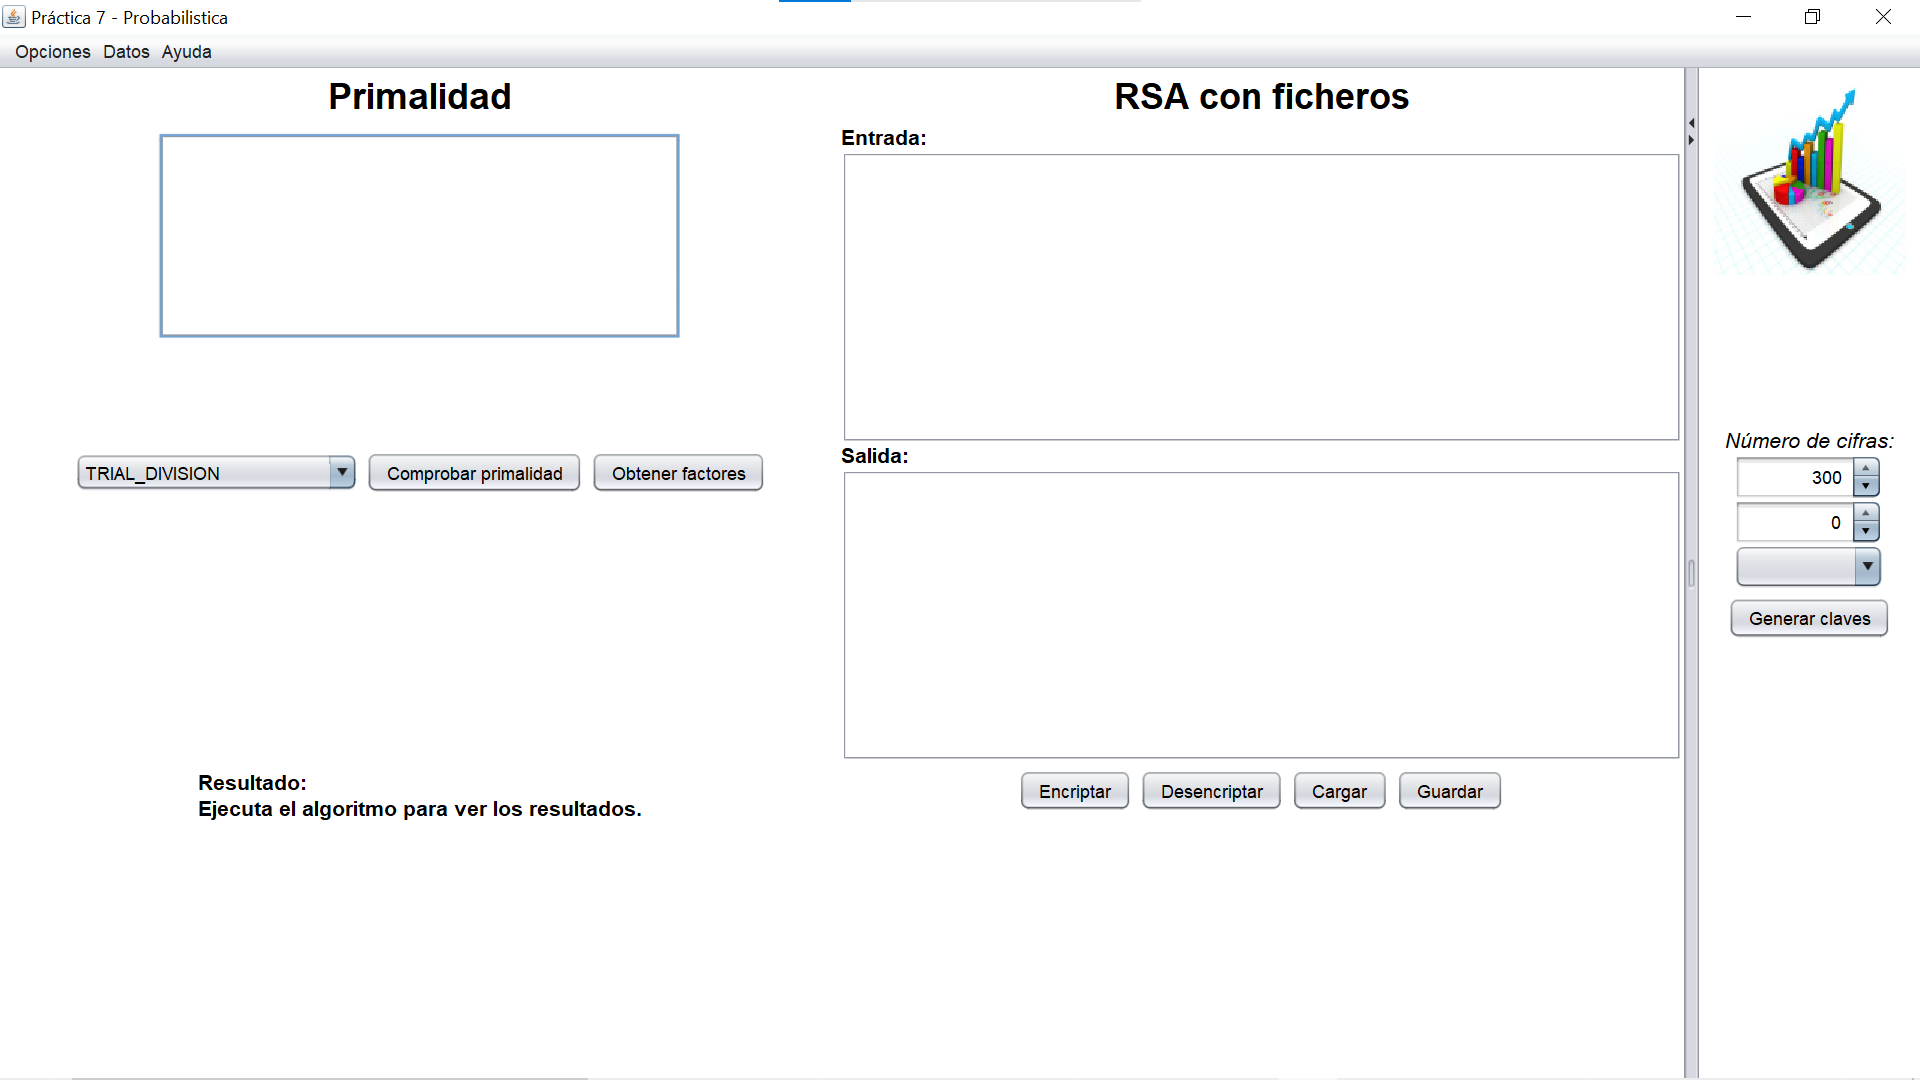
\includegraphics[width=\linewidth]{Usage/img/GUI.png}
    \caption{Interfaz de usuario}
    \label{fig:User_interface}
\end{figure}

\subsection{Header}\label{Manual usuario, Header}
En el \say{header} de la aplicación podemos encontrar un conjunto de botones con imágenes que nos permiten seleccionar las piezas para poner sobre el tablero. Cuando se seleccione una pieza, ésta se verá reflejada en el cursor y se podrá añadir en cualquier punto del tablero clicando sobre una casilla. \bigskip

Los botones del \say{header} para seleccionar las piezas, de izquierda a derecha, son: 

\begin{multicols}{2}
\begin{itemize}
    \item[] Rey
    \item[] Reina
    \item[] Torre
    \item[] Caballo
    \item[] Álfil
    \item[] Unicornio
    \item[] Dragon
    \item[] Castillo
\end{itemize}
\end{multicols}

\subsection{Main}
En el principal bloque de la aplicación se encuentra el tablero donde se ejecutará el algoritmo de backtracking. En esta sección, se representa el tamaño del tablero, las piezas que hay en el tablero y las casillas. \bigskip

Añadir que en la parte derecha del tablero se podrán consultar las estadísticas, donde se da información acerca del tamaño del tablero, piezas que hay sobre el tablero, tiempo transcurrido y progreso del algoritmo. 

\subsection{Sidebar}
En el \say{Sidebar} de la apliación se encuentran las estadísticas del de la ejecución. En estas estadísticas se indica el tamaño del tablero, el número de piezas que hay sobre el tablero, el tiempo transcurrido en encontrar la solución y el progreso del algoritmo se verá reflejado en la barra de progreso.

\subsection{Footer}
En el \say{footer} de la aplicación se pueden encontrar un conjunto de \say{gadgets} que nos permiten controlar la ejecución del programa y visualización. A continuación se explicará cada uno de ellos de izquierda a derecha: \bigskip

Primeramente, el botón definido por la etiqueta \say{Iniciar} permite iniciar el algoritmo con la configuración que el usuario haya elegido, es decir, se iniciará con el tamaño del tablero seleccionado y con N piezas sobre el tablero que el usuario habrá indicado donde comienza cada una. Si se pulsa el botón \say{Iniciar} sin que haya ninguna pieza sobre el tablero, saltará un Error diciendo que no hay piezas suficientes piezas en el tablero.  \bigskip

Por otra parte, el botón definido por la etiqueta \say{Reiniciar} permite reiniciar el algoritmo y el tablero y dejarlo como al principio de la ejecución del programa. El usuario deberá introducir otra configuración de piezas y de tamaño de tablero para volverlo a ejecutar.  \bigskip

Por último, a la derecha de éste hay un objeto JSpinner para seleccionar el \say{Tamaño del tablero}, cada vez que se cambie el tamaño del tablero, el cambio se verá reflejado sobre el tablero representado por pantalla. Como mínimo, el tablero tiene que ser de 2x2 y como máximo 32x32. Queda claro que el algoritmo tardará menos en ejecutarse en un tablero de 2x2 que en un tablero de 32x32, ya que se tienen que recorrer muchos menos puntos.

\subsection{Ejemplo ejecución}

Al iniciar la aplicación se mostrará una interfaz como la expuesta en la imagen \ref{fig:User_interface}. Para poder iniciar la ejecución del algoritmo, es necesario que se coloquen 1 o más piezas en el tablero de diferentes tipos, como se ha mencionado anteriormente en la sección \ref{Manual usuario, Header}. Una vez ya seleccionada las N fichas, se debe pulsar el botón de iniciar, provacando que se inicie el algoritmo y viendo a tiempo real la ejecución del \say{backtracking}, junto a los datos de la ejecución a la derecha.\bigskip

A continuación, la siguiente imagen, muestra un ejemplo de la interfaz en mitad de la ejecución:

\begin{figure}[!h]
    \centering
    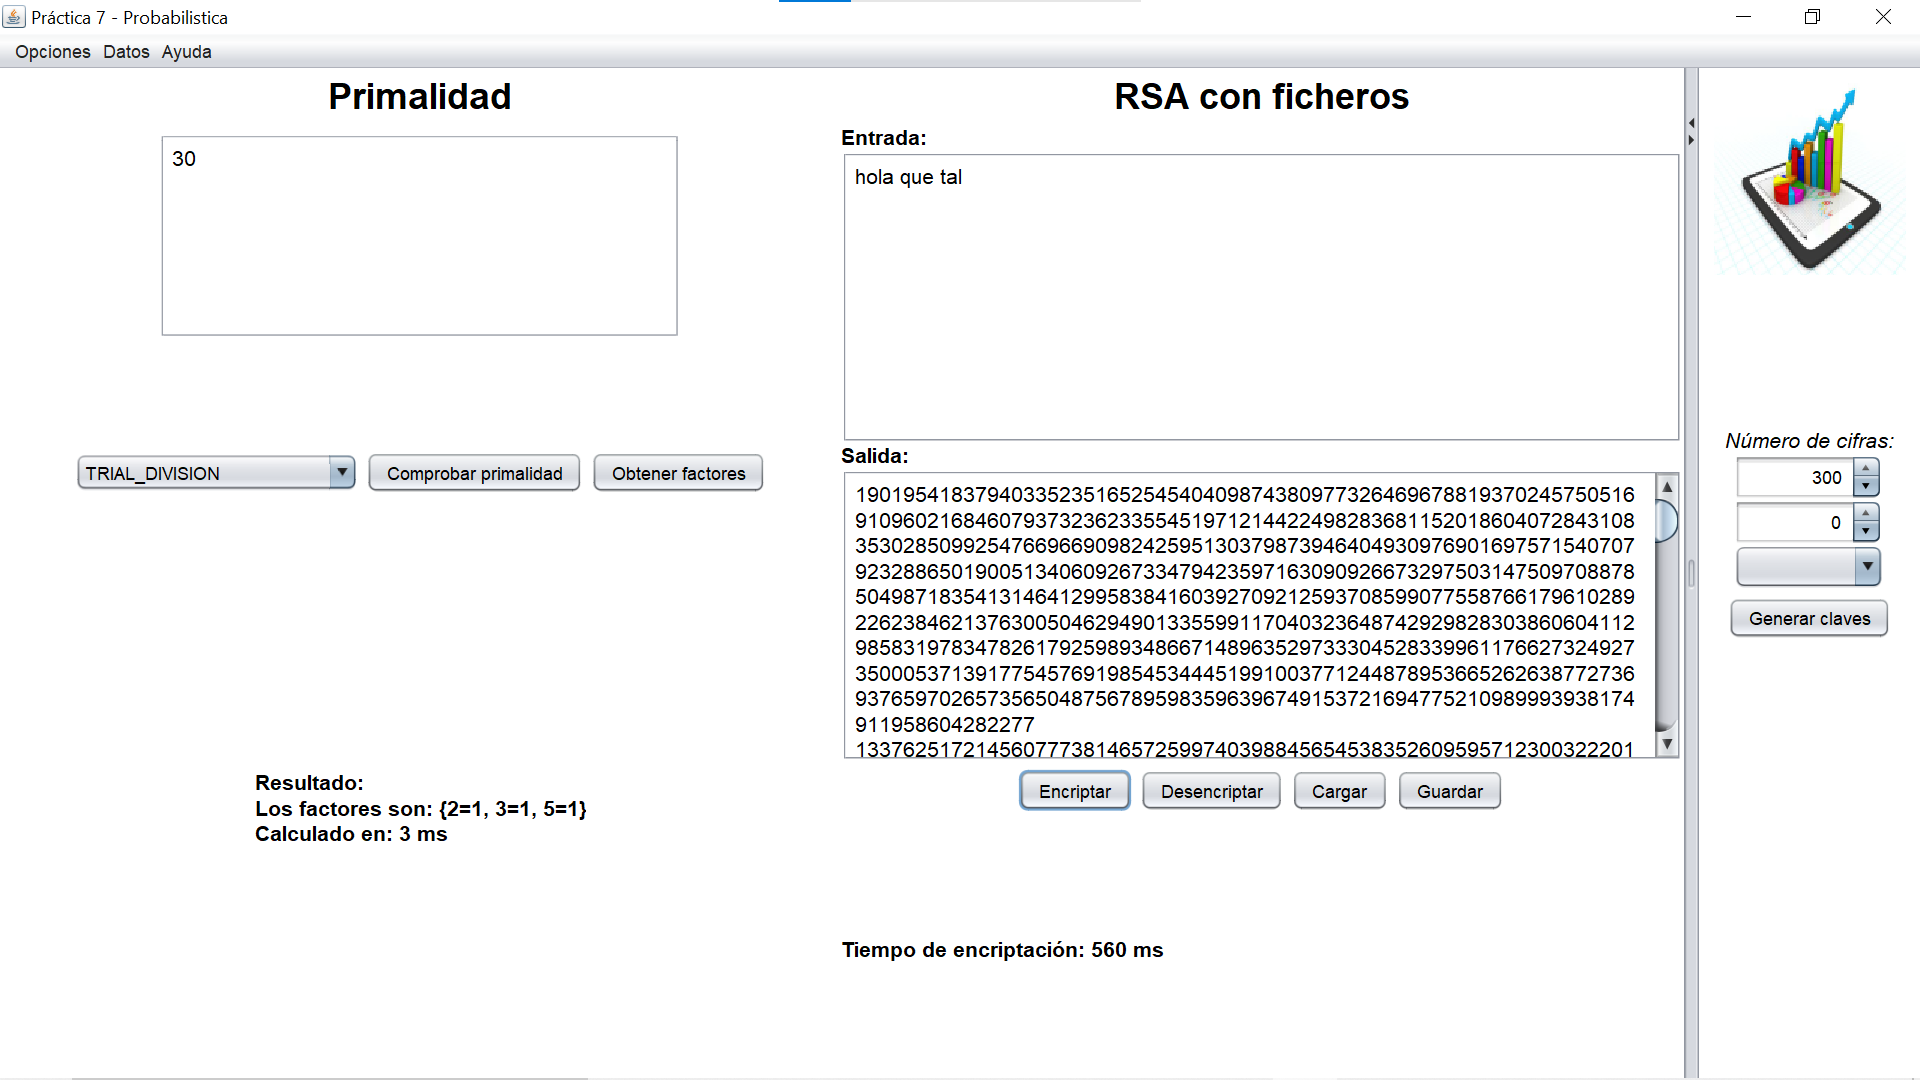
\includegraphics[width=\linewidth]{Usage/img/ejecucion.png}
    \caption{Interfaz de usuario}
    \label{fig:Ejemplo ejecución}
\end{figure}

A partir de aqui, el usuario puede reiniciar la ejecución para ejecutar nuevamente el algoritmo.
\section{Manual de usuario}\label{Manual usuario}

Para el correcto uso de la aplicación, el conjunto de acciones que se pueden realizar en dicho programa serán definidas a continuación. También, la distribución de las secciones de la interfaz junto a su explicación y funcionalidad.\bigskip

Cuando se ejecute el programa por primera vez en la pantalla se debe mostrar la siguiente interfaz de usuario:

\begin{figure}[!h]
    \centering
    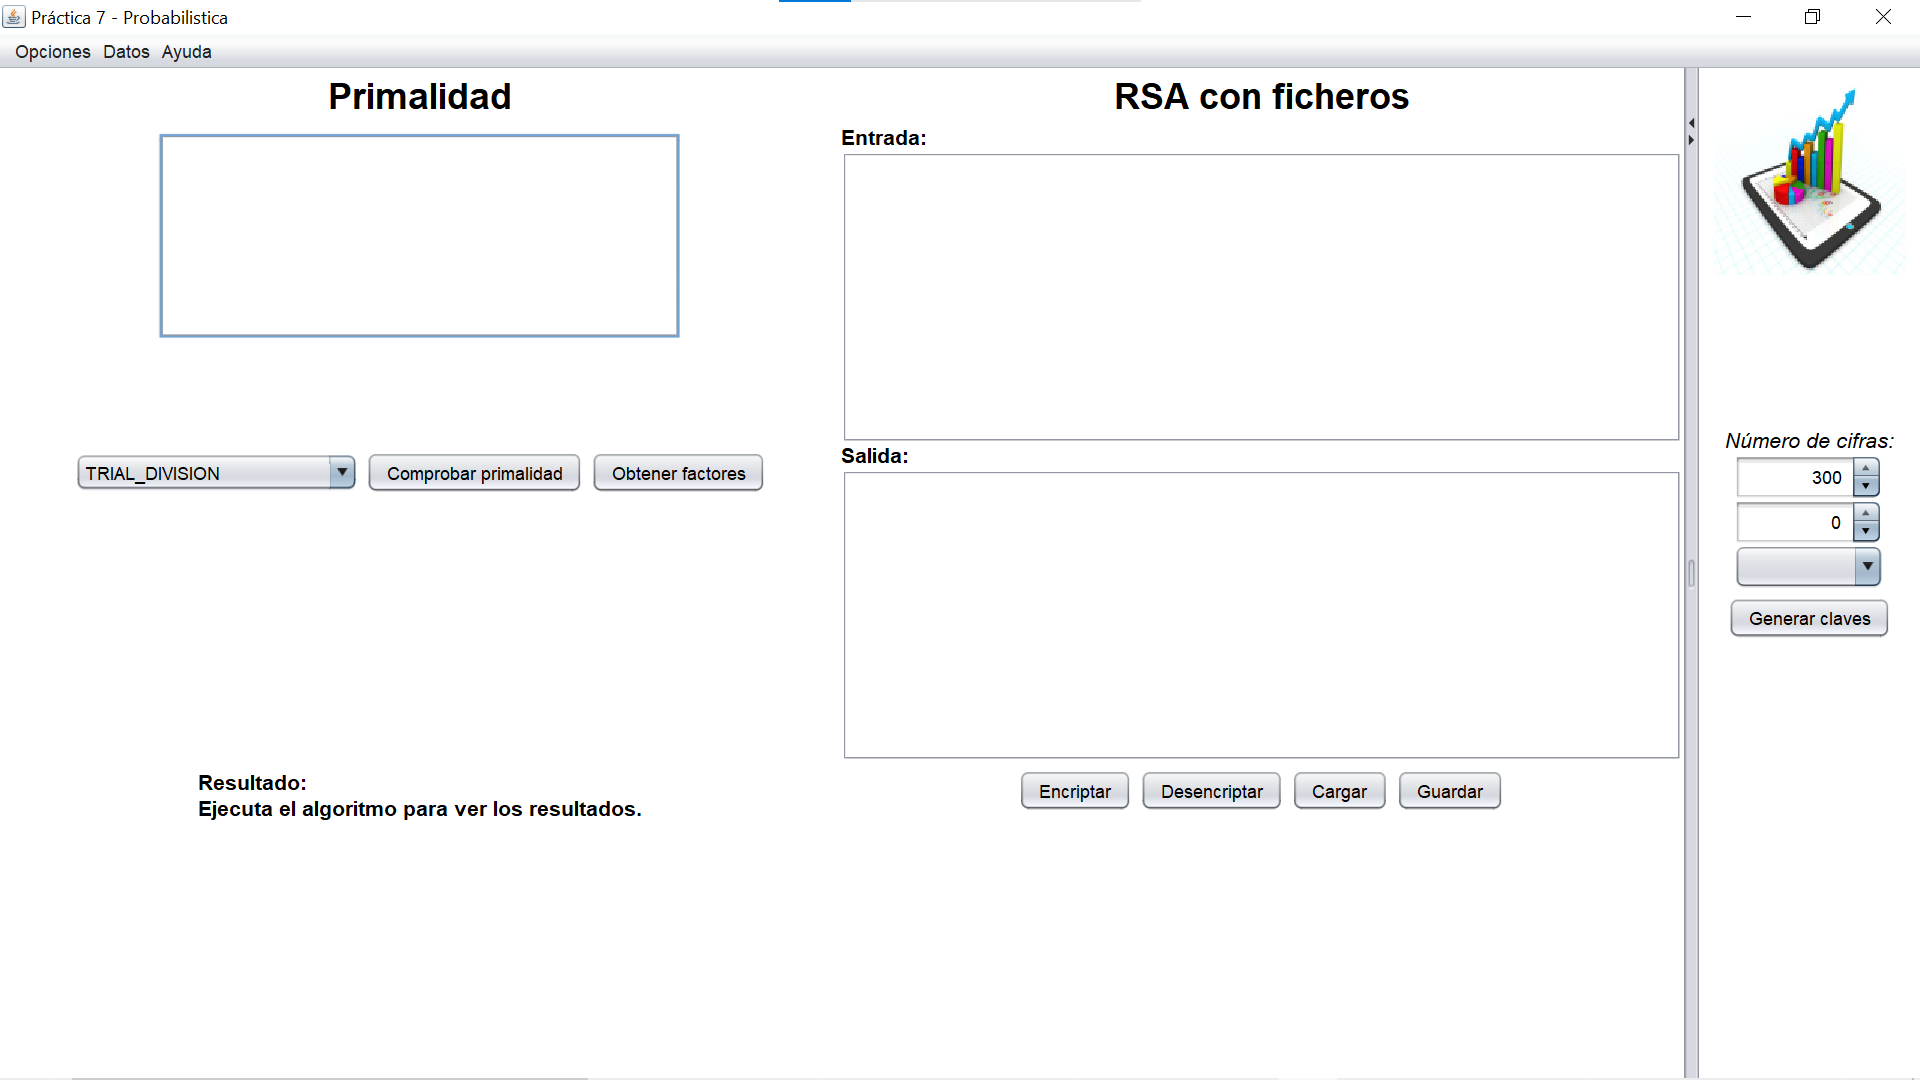
\includegraphics[width=\linewidth]{Usage/img/GUI.png}
    \caption{Interfaz de usuario}
    \label{fig:User_interface}
\end{figure}

\subsection{Header}\label{Manual usuario, Header}
En el \say{header} de la aplicación podemos encontrar un conjunto de botones con imágenes que nos permiten seleccionar las piezas para poner sobre el tablero. Cuando se seleccione una pieza, ésta se verá reflejada en el cursor y se podrá añadir en cualquier punto del tablero clicando sobre una casilla. \bigskip

Los botones del \say{header} para seleccionar las piezas, de izquierda a derecha, son: 

\begin{multicols}{2}
\begin{itemize}
    \item[] Rey
    \item[] Reina
    \item[] Torre
    \item[] Caballo
    \item[] Álfil
    \item[] Unicornio
    \item[] Dragon
    \item[] Castillo
\end{itemize}
\end{multicols}

\subsection{Main}
En el principal bloque de la aplicación se encuentra el tablero donde se ejecutará el algoritmo de backtracking. En esta sección, se representa el tamaño del tablero, las piezas que hay en el tablero y las casillas. \bigskip

Añadir que en la parte derecha del tablero se podrán consultar las estadísticas, donde se da información acerca del tamaño del tablero, piezas que hay sobre el tablero, tiempo transcurrido y progreso del algoritmo. 

\subsection{Sidebar}
En el \say{Sidebar} de la apliación se encuentran las estadísticas del de la ejecución. En estas estadísticas se indica el tamaño del tablero, el número de piezas que hay sobre el tablero, el tiempo transcurrido en encontrar la solución y el progreso del algoritmo se verá reflejado en la barra de progreso.

\subsection{Footer}
En el \say{footer} de la aplicación se pueden encontrar un conjunto de \say{gadgets} que nos permiten controlar la ejecución del programa y visualización. A continuación se explicará cada uno de ellos de izquierda a derecha: \bigskip

Primeramente, el botón definido por la etiqueta \say{Iniciar} permite iniciar el algoritmo con la configuración que el usuario haya elegido, es decir, se iniciará con el tamaño del tablero seleccionado y con N piezas sobre el tablero que el usuario habrá indicado donde comienza cada una. Si se pulsa el botón \say{Iniciar} sin que haya ninguna pieza sobre el tablero, saltará un Error diciendo que no hay piezas suficientes piezas en el tablero.  \bigskip

Por otra parte, el botón definido por la etiqueta \say{Reiniciar} permite reiniciar el algoritmo y el tablero y dejarlo como al principio de la ejecución del programa. El usuario deberá introducir otra configuración de piezas y de tamaño de tablero para volverlo a ejecutar.  \bigskip

Por último, a la derecha de éste hay un objeto JSpinner para seleccionar el \say{Tamaño del tablero}, cada vez que se cambie el tamaño del tablero, el cambio se verá reflejado sobre el tablero representado por pantalla. Como mínimo, el tablero tiene que ser de 2x2 y como máximo 32x32. Queda claro que el algoritmo tardará menos en ejecutarse en un tablero de 2x2 que en un tablero de 32x32, ya que se tienen que recorrer muchos menos puntos.

\subsection{Ejemplo ejecución}

Al iniciar la aplicación se mostrará una interfaz como la expuesta en la imagen \ref{fig:User_interface}. Para poder iniciar la ejecución del algoritmo, es necesario que se coloquen 1 o más piezas en el tablero de diferentes tipos, como se ha mencionado anteriormente en la sección \ref{Manual usuario, Header}. Una vez ya seleccionada las N fichas, se debe pulsar el botón de iniciar, provacando que se inicie el algoritmo y viendo a tiempo real la ejecución del \say{backtracking}, junto a los datos de la ejecución a la derecha.\bigskip

A continuación, la siguiente imagen, muestra un ejemplo de la interfaz en mitad de la ejecución:

\begin{figure}[!h]
    \centering
    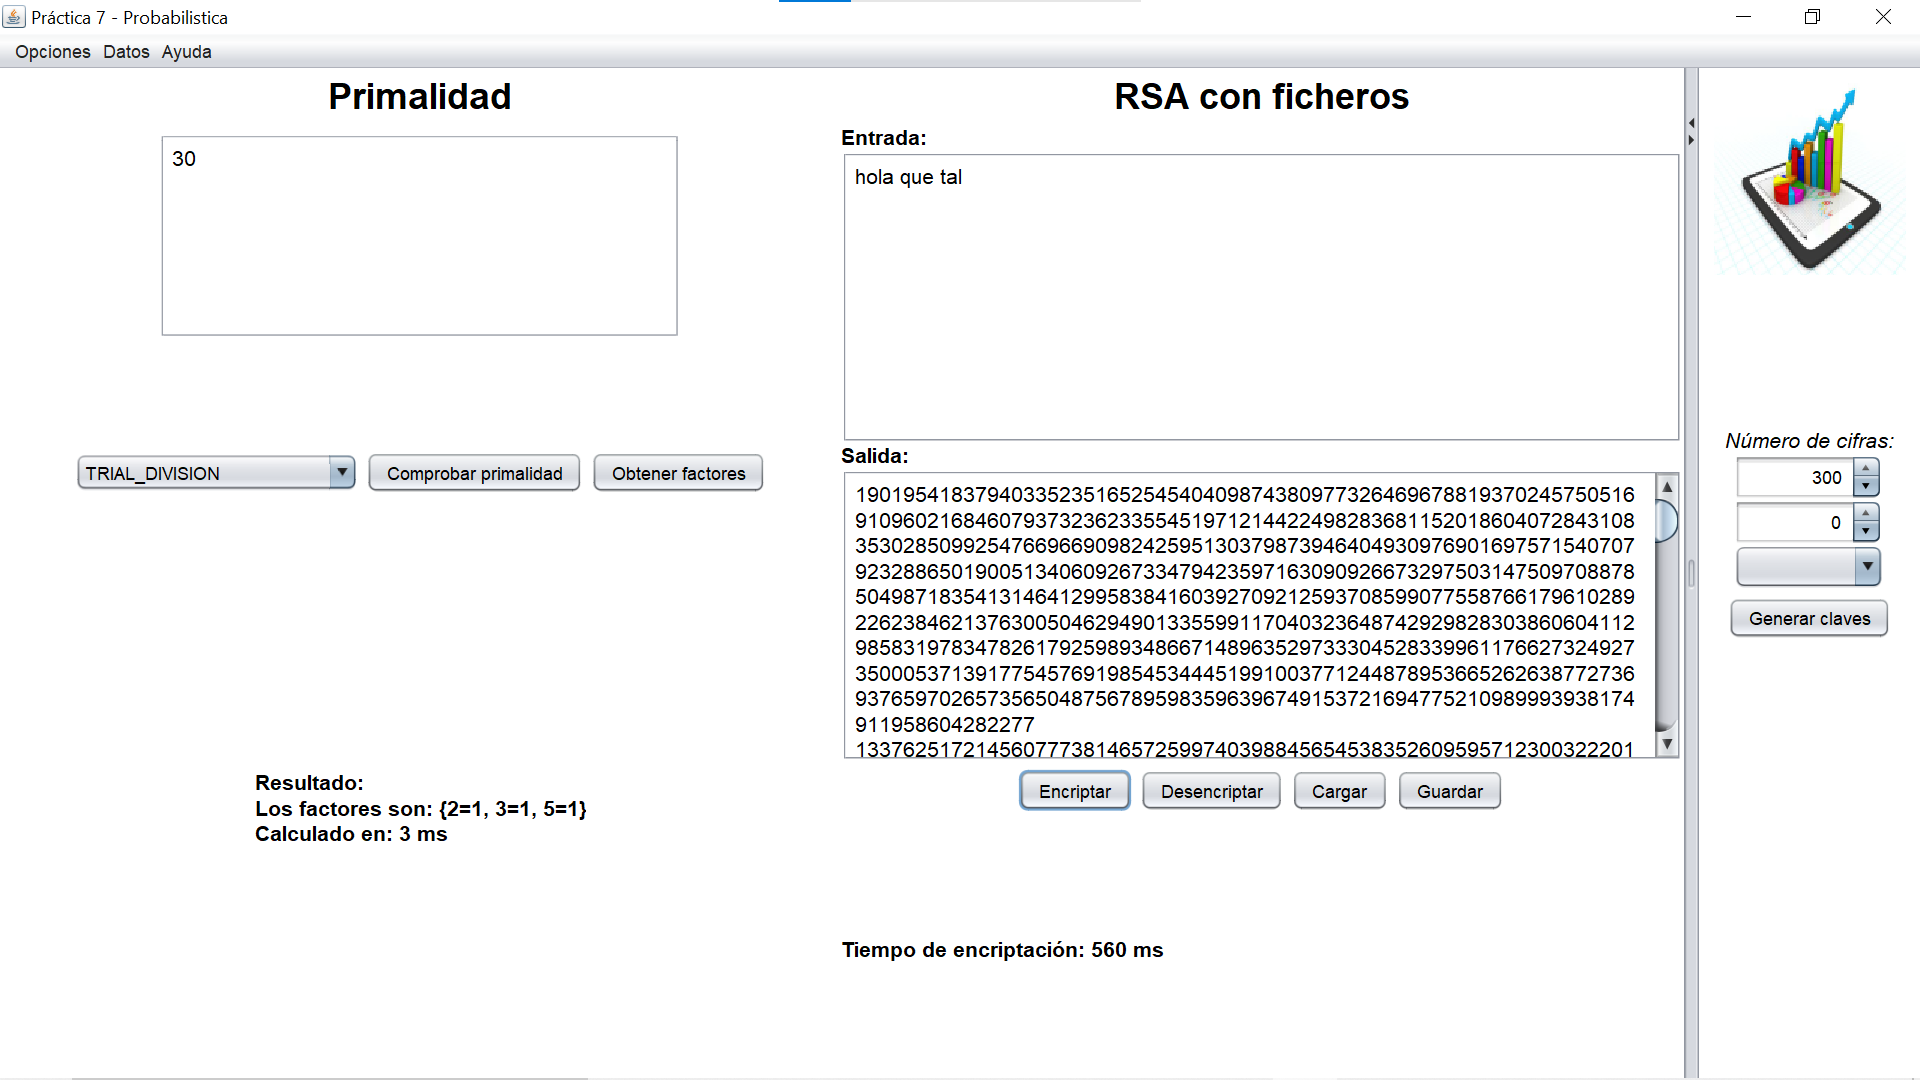
\includegraphics[width=\linewidth]{Usage/img/ejecucion.png}
    \caption{Interfaz de usuario}
    \label{fig:Ejemplo ejecución}
\end{figure}

A partir de aqui, el usuario puede reiniciar la ejecución para ejecutar nuevamente el algoritmo.
\section{Manual de usuario}\label{Manual usuario}

Para el correcto uso de la aplicación, el conjunto de acciones que se pueden realizar en dicho programa serán definidas a continuación. También, la distribución de las secciones de la interfaz junto a su explicación y funcionalidad.\bigskip

Cuando se ejecute el programa por primera vez en la pantalla se debe mostrar la siguiente interfaz de usuario:

\begin{figure}[!h]
    \centering
    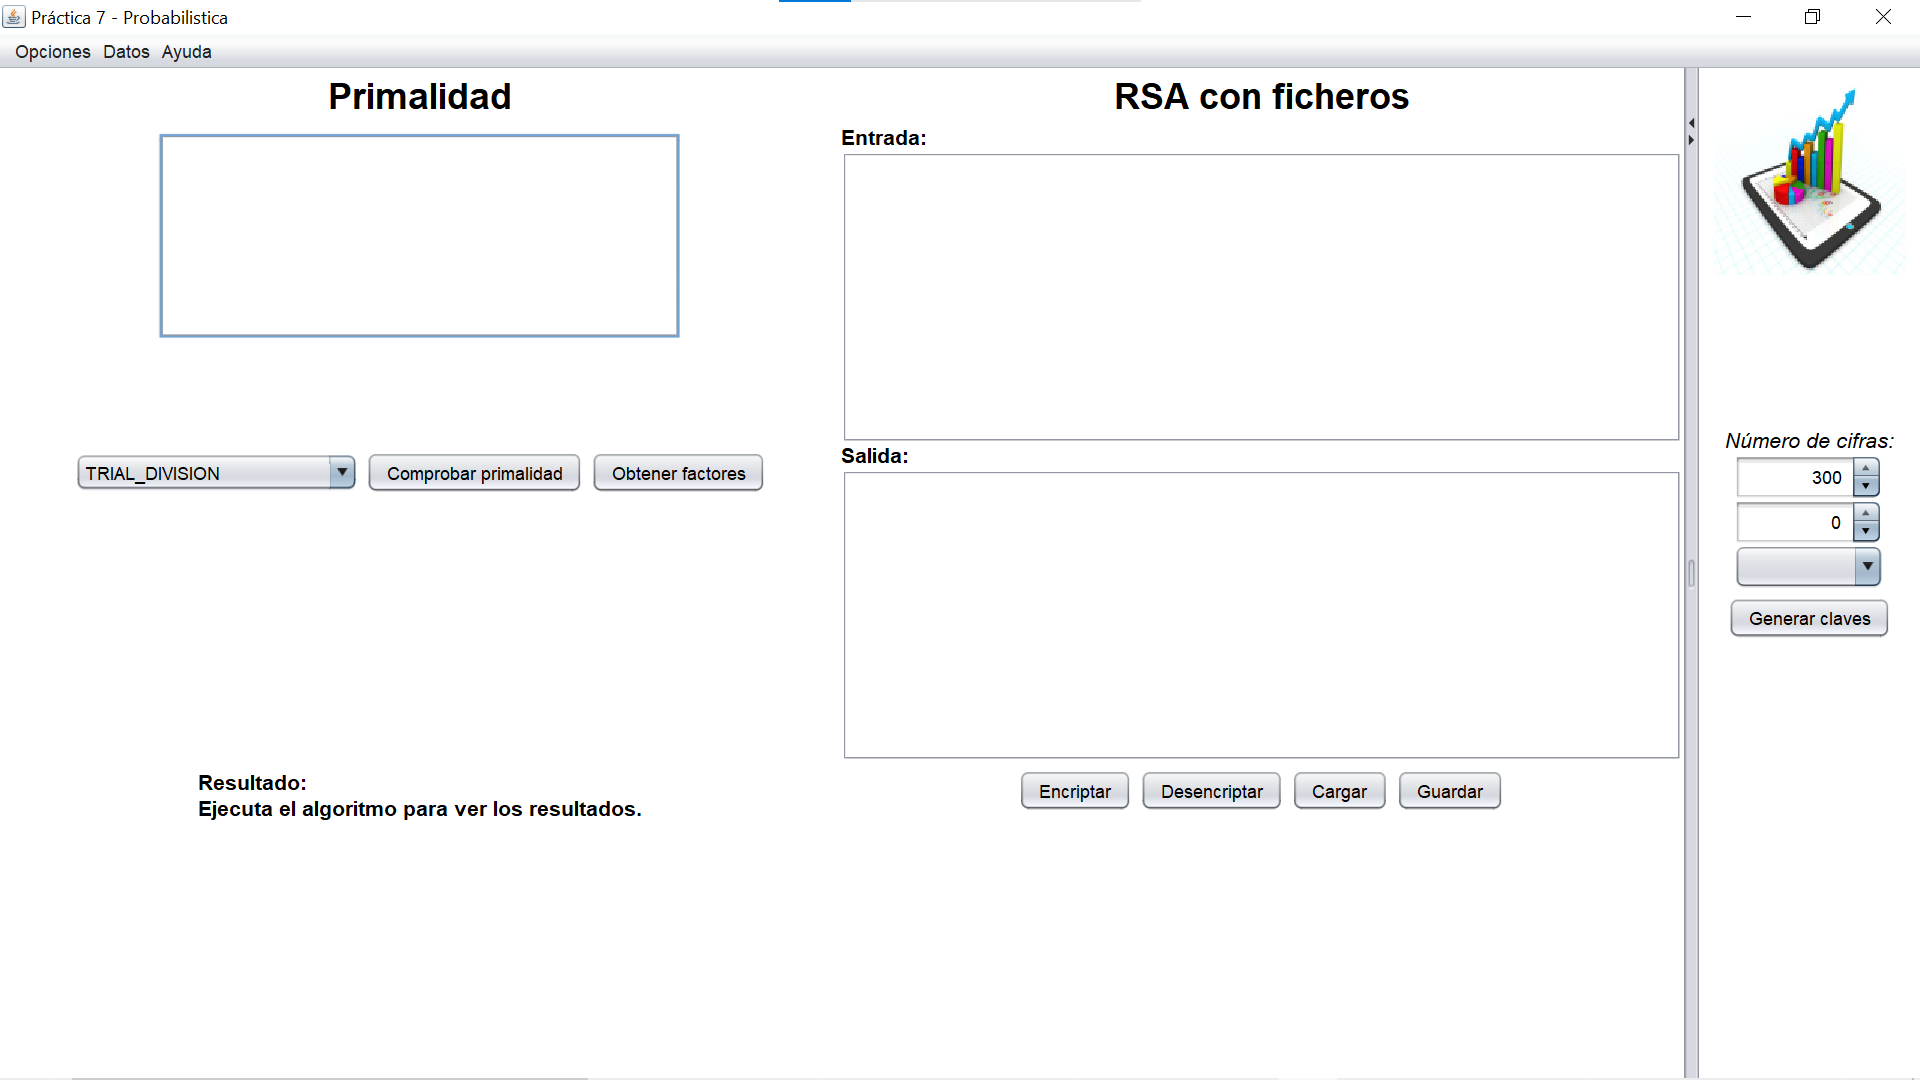
\includegraphics[width=\linewidth]{Usage/img/GUI.png}
    \caption{Interfaz de usuario}
    \label{fig:User_interface}
\end{figure}

\subsection{Header}\label{Manual usuario, Header}
En el \say{header} de la aplicación podemos encontrar un conjunto de botones con imágenes que nos permiten seleccionar las piezas para poner sobre el tablero. Cuando se seleccione una pieza, ésta se verá reflejada en el cursor y se podrá añadir en cualquier punto del tablero clicando sobre una casilla. \bigskip

Los botones del \say{header} para seleccionar las piezas, de izquierda a derecha, son: 

\begin{multicols}{2}
\begin{itemize}
    \item[] Rey
    \item[] Reina
    \item[] Torre
    \item[] Caballo
    \item[] Álfil
    \item[] Unicornio
    \item[] Dragon
    \item[] Castillo
\end{itemize}
\end{multicols}

\subsection{Main}
En el principal bloque de la aplicación se encuentra el tablero donde se ejecutará el algoritmo de backtracking. En esta sección, se representa el tamaño del tablero, las piezas que hay en el tablero y las casillas. \bigskip

Añadir que en la parte derecha del tablero se podrán consultar las estadísticas, donde se da información acerca del tamaño del tablero, piezas que hay sobre el tablero, tiempo transcurrido y progreso del algoritmo. 

\subsection{Sidebar}
En el \say{Sidebar} de la apliación se encuentran las estadísticas del de la ejecución. En estas estadísticas se indica el tamaño del tablero, el número de piezas que hay sobre el tablero, el tiempo transcurrido en encontrar la solución y el progreso del algoritmo se verá reflejado en la barra de progreso.

\subsection{Footer}
En el \say{footer} de la aplicación se pueden encontrar un conjunto de \say{gadgets} que nos permiten controlar la ejecución del programa y visualización. A continuación se explicará cada uno de ellos de izquierda a derecha: \bigskip

Primeramente, el botón definido por la etiqueta \say{Iniciar} permite iniciar el algoritmo con la configuración que el usuario haya elegido, es decir, se iniciará con el tamaño del tablero seleccionado y con N piezas sobre el tablero que el usuario habrá indicado donde comienza cada una. Si se pulsa el botón \say{Iniciar} sin que haya ninguna pieza sobre el tablero, saltará un Error diciendo que no hay piezas suficientes piezas en el tablero.  \bigskip

Por otra parte, el botón definido por la etiqueta \say{Reiniciar} permite reiniciar el algoritmo y el tablero y dejarlo como al principio de la ejecución del programa. El usuario deberá introducir otra configuración de piezas y de tamaño de tablero para volverlo a ejecutar.  \bigskip

Por último, a la derecha de éste hay un objeto JSpinner para seleccionar el \say{Tamaño del tablero}, cada vez que se cambie el tamaño del tablero, el cambio se verá reflejado sobre el tablero representado por pantalla. Como mínimo, el tablero tiene que ser de 2x2 y como máximo 32x32. Queda claro que el algoritmo tardará menos en ejecutarse en un tablero de 2x2 que en un tablero de 32x32, ya que se tienen que recorrer muchos menos puntos.

\subsection{Ejemplo ejecución}

Al iniciar la aplicación se mostrará una interfaz como la expuesta en la imagen \ref{fig:User_interface}. Para poder iniciar la ejecución del algoritmo, es necesario que se coloquen 1 o más piezas en el tablero de diferentes tipos, como se ha mencionado anteriormente en la sección \ref{Manual usuario, Header}. Una vez ya seleccionada las N fichas, se debe pulsar el botón de iniciar, provacando que se inicie el algoritmo y viendo a tiempo real la ejecución del \say{backtracking}, junto a los datos de la ejecución a la derecha.\bigskip

A continuación, la siguiente imagen, muestra un ejemplo de la interfaz en mitad de la ejecución:

\begin{figure}[!h]
    \centering
    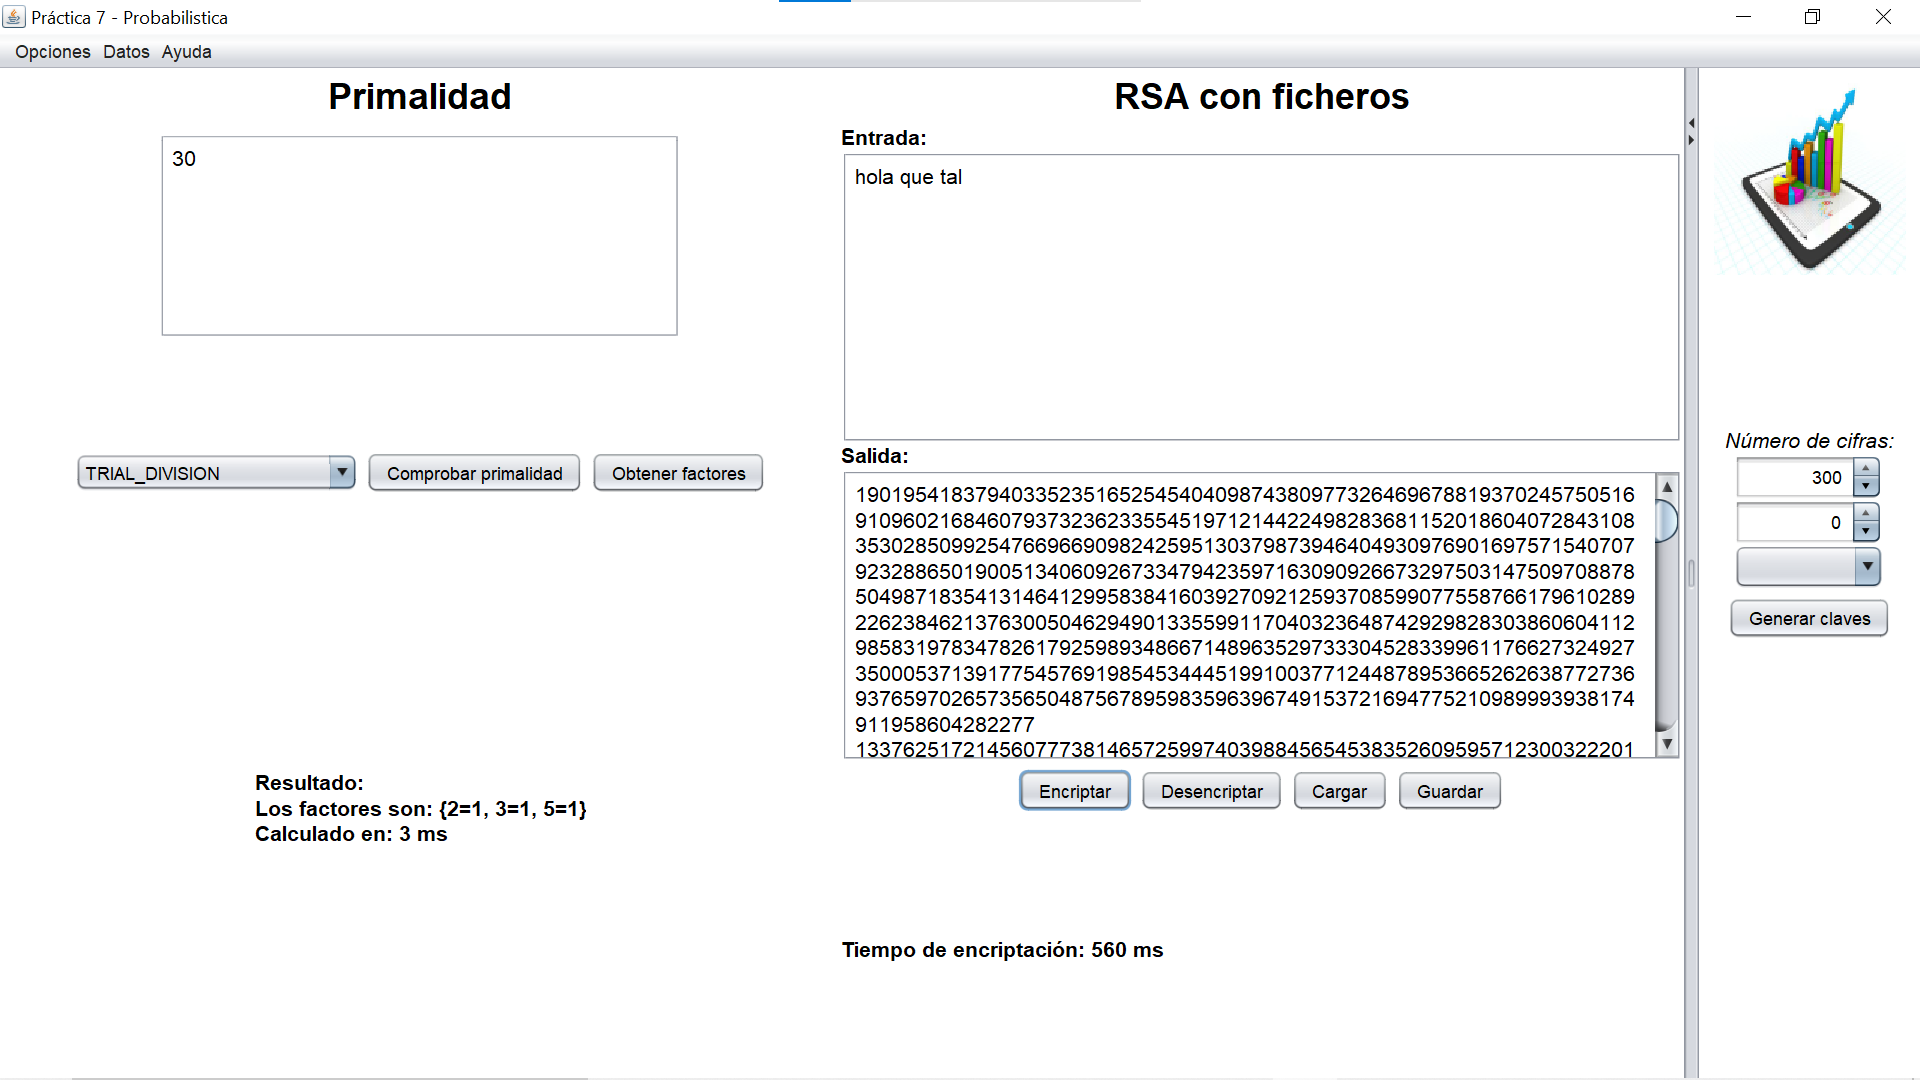
\includegraphics[width=\linewidth]{Usage/img/ejecucion.png}
    \caption{Interfaz de usuario}
    \label{fig:Ejemplo ejecución}
\end{figure}

A partir de aqui, el usuario puede reiniciar la ejecución para ejecutar nuevamente el algoritmo.
\section{Manual de usuario}\label{Manual usuario}

Para el correcto uso de la aplicación, el conjunto de acciones que se pueden realizar en dicho programa serán definidas a continuación. También, la distribución de las secciones de la interfaz junto a su explicación y funcionalidad.\bigskip

Cuando se ejecute el programa por primera vez en la pantalla se debe mostrar la siguiente interfaz de usuario:

\begin{figure}[!h]
    \centering
    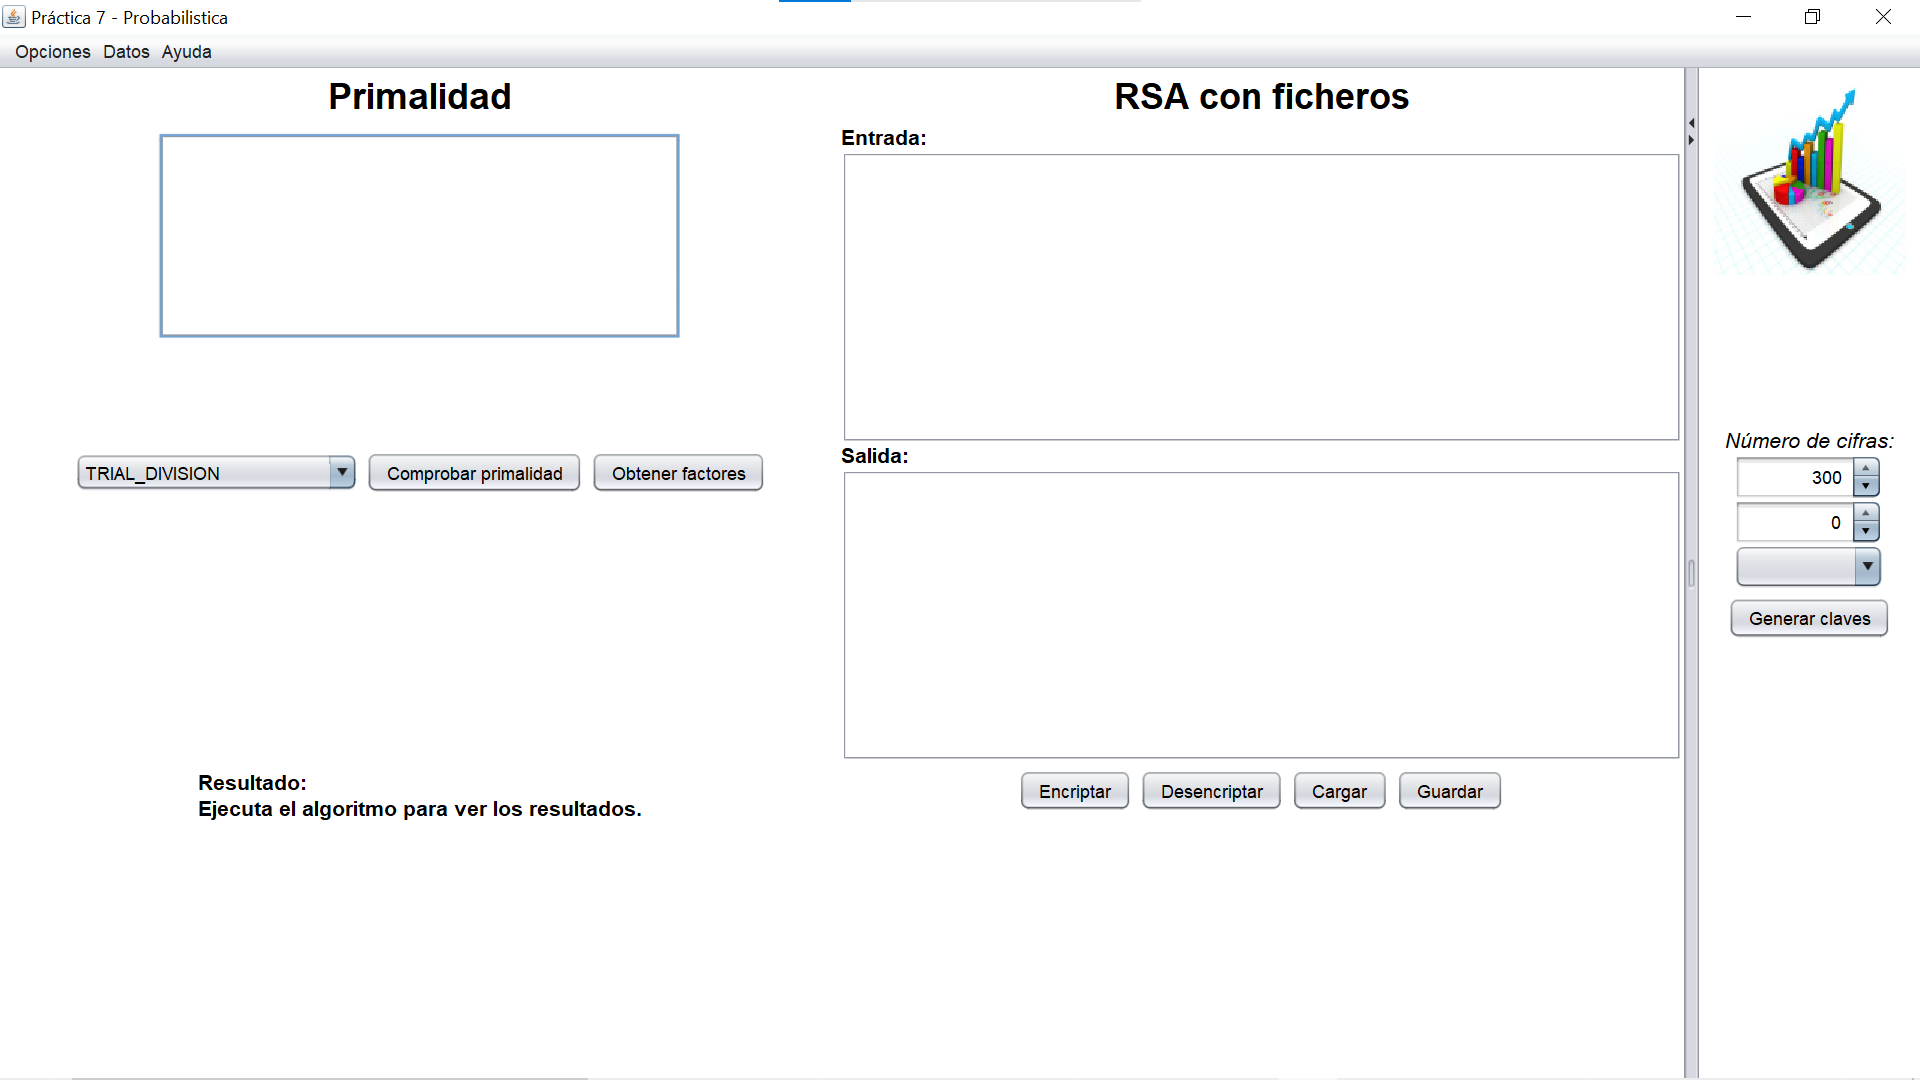
\includegraphics[width=\linewidth]{Usage/img/GUI.png}
    \caption{Interfaz de usuario}
    \label{fig:User_interface}
\end{figure}

\subsection{Header}\label{Manual usuario, Header}
En el \say{header} de la aplicación podemos encontrar un conjunto de botones con imágenes que nos permiten seleccionar las piezas para poner sobre el tablero. Cuando se seleccione una pieza, ésta se verá reflejada en el cursor y se podrá añadir en cualquier punto del tablero clicando sobre una casilla. \bigskip

Los botones del \say{header} para seleccionar las piezas, de izquierda a derecha, son: 

\begin{multicols}{2}
\begin{itemize}
    \item[] Rey
    \item[] Reina
    \item[] Torre
    \item[] Caballo
    \item[] Álfil
    \item[] Unicornio
    \item[] Dragon
    \item[] Castillo
\end{itemize}
\end{multicols}

\subsection{Main}
En el principal bloque de la aplicación se encuentra el tablero donde se ejecutará el algoritmo de backtracking. En esta sección, se representa el tamaño del tablero, las piezas que hay en el tablero y las casillas. \bigskip

Añadir que en la parte derecha del tablero se podrán consultar las estadísticas, donde se da información acerca del tamaño del tablero, piezas que hay sobre el tablero, tiempo transcurrido y progreso del algoritmo. 

\subsection{Sidebar}
En el \say{Sidebar} de la apliación se encuentran las estadísticas del de la ejecución. En estas estadísticas se indica el tamaño del tablero, el número de piezas que hay sobre el tablero, el tiempo transcurrido en encontrar la solución y el progreso del algoritmo se verá reflejado en la barra de progreso.

\subsection{Footer}
En el \say{footer} de la aplicación se pueden encontrar un conjunto de \say{gadgets} que nos permiten controlar la ejecución del programa y visualización. A continuación se explicará cada uno de ellos de izquierda a derecha: \bigskip

Primeramente, el botón definido por la etiqueta \say{Iniciar} permite iniciar el algoritmo con la configuración que el usuario haya elegido, es decir, se iniciará con el tamaño del tablero seleccionado y con N piezas sobre el tablero que el usuario habrá indicado donde comienza cada una. Si se pulsa el botón \say{Iniciar} sin que haya ninguna pieza sobre el tablero, saltará un Error diciendo que no hay piezas suficientes piezas en el tablero.  \bigskip

Por otra parte, el botón definido por la etiqueta \say{Reiniciar} permite reiniciar el algoritmo y el tablero y dejarlo como al principio de la ejecución del programa. El usuario deberá introducir otra configuración de piezas y de tamaño de tablero para volverlo a ejecutar.  \bigskip

Por último, a la derecha de éste hay un objeto JSpinner para seleccionar el \say{Tamaño del tablero}, cada vez que se cambie el tamaño del tablero, el cambio se verá reflejado sobre el tablero representado por pantalla. Como mínimo, el tablero tiene que ser de 2x2 y como máximo 32x32. Queda claro que el algoritmo tardará menos en ejecutarse en un tablero de 2x2 que en un tablero de 32x32, ya que se tienen que recorrer muchos menos puntos.

\subsection{Ejemplo ejecución}

Al iniciar la aplicación se mostrará una interfaz como la expuesta en la imagen \ref{fig:User_interface}. Para poder iniciar la ejecución del algoritmo, es necesario que se coloquen 1 o más piezas en el tablero de diferentes tipos, como se ha mencionado anteriormente en la sección \ref{Manual usuario, Header}. Una vez ya seleccionada las N fichas, se debe pulsar el botón de iniciar, provacando que se inicie el algoritmo y viendo a tiempo real la ejecución del \say{backtracking}, junto a los datos de la ejecución a la derecha.\bigskip

A continuación, la siguiente imagen, muestra un ejemplo de la interfaz en mitad de la ejecución:

\begin{figure}[!h]
    \centering
    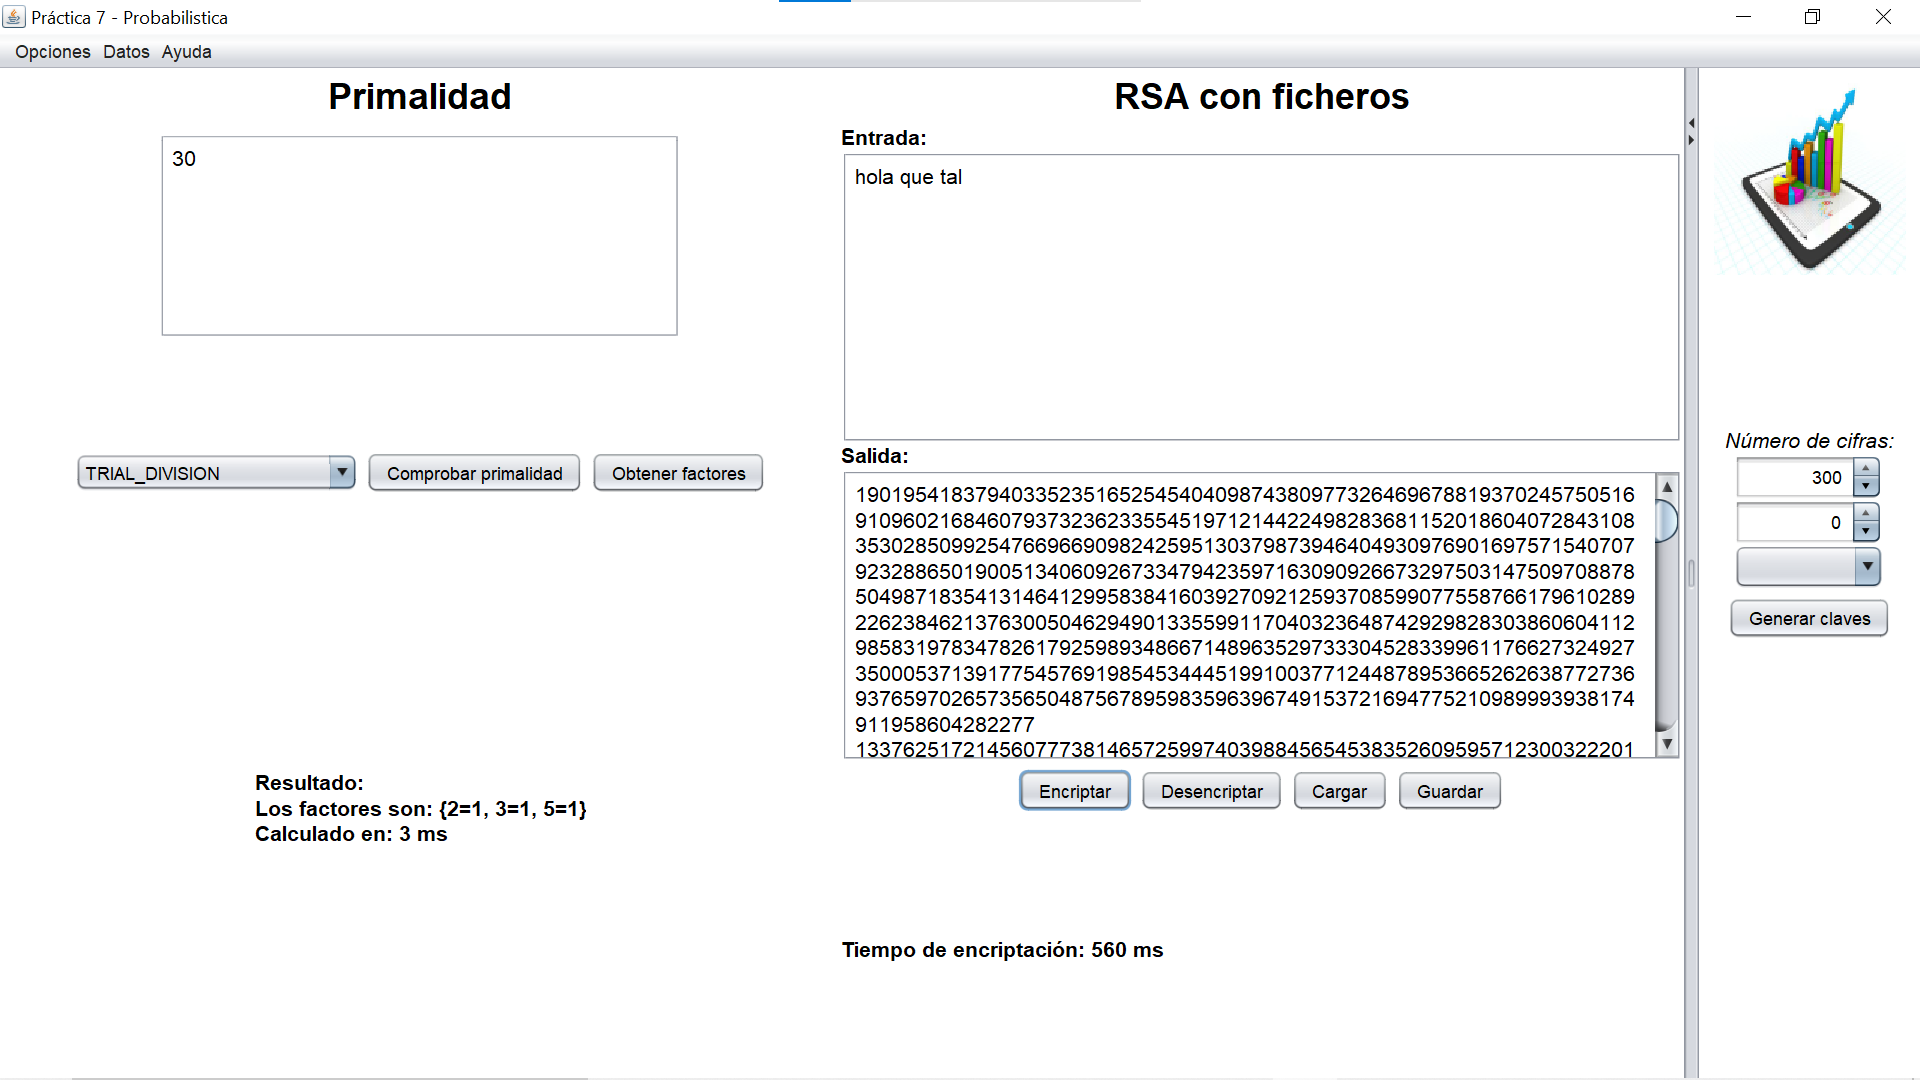
\includegraphics[width=\linewidth]{Usage/img/ejecucion.png}
    \caption{Interfaz de usuario}
    \label{fig:Ejemplo ejecución}
\end{figure}

A partir de aqui, el usuario puede reiniciar la ejecución para ejecutar nuevamente el algoritmo.
\section{Distribución del trabajo realizado}

El trabajo realizado por cada miembro de la práctica ha sido el siguiente: \bigskip

\begin{itemize}
    \item Alejandro Rodríguez:
    \begin{itemize}
        \item Documentación
        \item Diseño del proyecto
        \item Desarrollador de la base del \say{Language guesser}
        \item Desarrollador de la plantilla base del proyecto
    \end{itemize}
    
    \item Rubén Palmer:
    \begin{itemize}
        \item Documentación
        \item Diseño del proyecto
        \item Principal desarrollador del \say{backend} de la aplicación
        \item Desarrollador general de la aplicación
        \item Desarrollador del \say{frontend}
        \item Diseñador de la implementación del patrón MVC de la aplicación
        \item Desarrollador de la plantilla base del proyecto
        \item Desarrollador de la plantilla de la documentación 
    \end{itemize}
    \item Sergi Mayol:
    \begin{itemize}
        \item Documentación
        \item Diseño del proyecto
        \item Desarrollador de la librería \texttt{Better Swing}
        \item Principal desarrollador del \say{frontend} de la aplicación
        \item Desarrollador general de la aplicación
        \item Desarrollador del \say{backend} de la aplicación
        \item Diseñador de la implementación del patrón MVC de la aplicación
        \item Desarrollador de la plantilla base del proyecto
    \end{itemize}
\end{itemize}

\begin{figure}[!h]
    \centering
    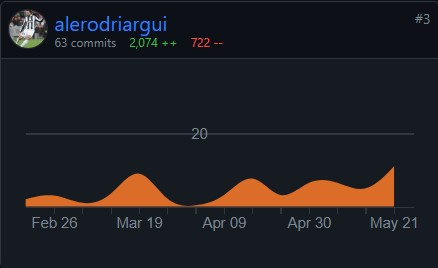
\includegraphics[width=\linewidth]{alex.png}
    \caption{Contribución en el proyecto de Alejandro Rodríguez}
    \label{fig:contrib_alex}
\end{figure}

\begin{figure}[!h]
    \centering
    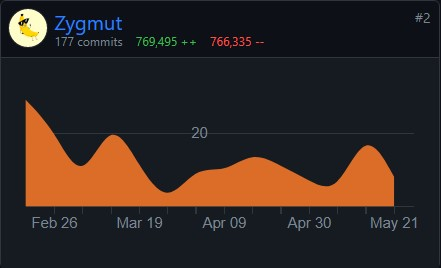
\includegraphics[width=\linewidth]{ruben.png}
    \caption{Contribución en el proyecto de Rubén Palmer}
    \label{fig:contrib_ruben}
\end{figure}

\begin{figure}[!h]
    \centering
    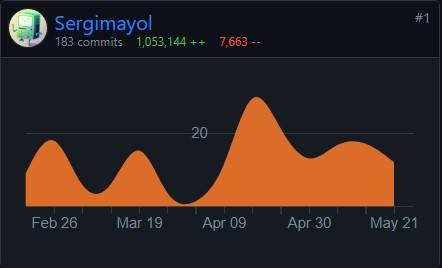
\includegraphics[width=\linewidth]{sergi.png}
    \caption{Contribución en el proyecto de Sergi Mayol}
    \label{fig:contrib_sergi}
\end{figure}

\newpage

% use section* for acknowledgment
\section*{Reconocimientos}
\begin{itemize}
    \item Se agradece la colaboración del Dr. Miquel Mascaró Portells en la resolución de dudas y supervisión del proyecto.
\end{itemize}

\begin{thebibliography}{1}

\bibitem{betterswing}
Better Swing, \emph{An easy way to develop java GUI apps}, V0.0.3. \hskip 1em plus
  0.5em minus 0.4em\relax Ver documentación completa \href{https://sergimayol.github.io/better-swing}{\textcolor{blue}{aquí}}.

\bibitem{Graphical engine}
Graphical engine, \emph{How to develop a graphical engine from scratch}. Ver enlace \href{https://www.youtube.com/watch?v=025QFeZfeyM&t=7334s}{\textcolor{blue}{aquí}}.

\bibitem{Gson}
Google json (Gson), \emph{Java serialization/deserialization library to convert Java Objects into JSON and back}. Ver enlace \href{https://github.com/google/gson}{\textcolor{blue}{aquí}}.

\bibitem{NodeJs architecture}
Node.js Architecture, \emph{Architecture of a single thread cross-platform, open-source server environment}. Ver enlace \href{https://codedamn.com/news/nodejs/node-js-architecture}{\textcolor{blue}{aquí}}.

\bibitem{Sqlite database}
The SQLite database, a serverless database. \emph{Quick start and documentation}. Ver enlace \href{https://www.sqlite.org/index.html}{\textcolor{blue}{aquí}}.

\bibitem{JFreeChart}
Open source Java chart library. \emph{An easy way to create and visualize charts in Java}. Ver enlace \href{https://www.jfree.org/jfreechart/}{\textcolor{blue}{aquí}}.

\bibitem{Method Overloading}
A way to define different behavior for a method with the same name. Ver enlace \href{https://www.geeksforgeeks.org/method-overloading-in-java/}{\textcolor{blue}{aquí}}.

\bibitem{RSA}
What is RSA? How does it work?. Ver enlace \href{https://es.wikipedia.org/wiki/RSA}{\textcolor{blue}{aquí}}.

\bibitem{Primality Test}
How to check if a number is prime. Ver enlace \href{https://en.wikipedia.org/wiki/Primality_test}{\textcolor{blue}{aquí}}.

\bibitem{Java BigInteger}
Java biginteger implementation and api docs reference. Ver enlace \href{https://docs.oracle.com/javase/8/docs/api/java/math/BigInteger.html}{\textcolor{blue}{aquí}}.

\bibitem{Pandas and Numpy}
Pandas and numpy for data analysis and visualization. Ver enlace Pandas: \href{https://pandas.pydata.org/}{\textcolor{blue}{aquí}}. Ver enlace Numpy: \href{https://numpy.org/}{\textcolor{blue}{aquí}} .

\bibitem{Jupyter Notebooks}
Jupyter notebooks for data analysis and visualization. Ver enlace \href{https://jupyter.org/}{\textcolor{blue}{aquí}}.

\bibitem{Trial division}
Trial division for integer factorization. Ver enlace \href{https://en.wikipedia.org/wiki/Trial_division}{\textcolor{blue}{aquí}}.

\bibitem{Fermat primality test}
Fermat primality test to determine whether a number is a probable prime. Ver enlace \href{https://en.wikipedia.org/wiki/Fermat_primality_test}{\textcolor{blue}{aquí}}.

\bibitem{Miller–Rabin primality test}
Miller–Rabin primality test to determine whether a number is a probable prime. Ver enlace \href{https://en.wikipedia.org/wiki/Miller%E2%80%93Rabin_primality_test}{\textcolor{blue}{aquí}}.

\bibitem{Thread pools in Java}
How to work with thread pools in Java. Ver enlace \href{https://www.baeldung.com/thread-pool-java-and-guava}{\textcolor{blue}{aquí}}.

\bibitem{Modular exponentiation}
Modular exponentiation. Ver enlace \href{https://en.wikipedia.org/wiki/Modular_exponentiation}{\textcolor{blue}{aquí}}.

\bibitem{Modular multiplicative inverse}
Modular multiplicative inverse. Ver enlace \href{https://en.wikipedia.org/wiki/Modular_multiplicative_inverse}{\textcolor{blue}{aquí}}.

\end{thebibliography}
\end{document}
